%%%%%%%%%%%%%%%%%%%%%%%%%%%%%%%%%%%%%%%%%%%%%%%%%%%%%%%%%%%%%%%%%%%%%%%%%
% ARTICLE ABOUT FATE OF SYNONYMOUS MUTATIONS IN HIV
%%%%%%%%%%%%%%%%%%%%%%%%%%%%%%%%%%%%%%%%%%%%%%%%%%%%%%%%%%%%%%%%%%%%%%%%%
\documentclass[rmp, twocolumn]{revtex4}
%%%%%%%%%%%%%%%%%%%%%%%%%%%%%%%%%%%%%%%%%%%%%%%%%%%%%%%%%%%%%%%%%%%%%%%%%
%%%%%%%%%%%%%%%%%%%%%%%%%%%%%%%%%%%%%%%%%%%%%%%%%%%%%%%%%%%%%%%%%%%%%%%%%
\usepackage[english]{babel}
\usepackage[utf8x]{inputenc}
\usepackage{amsmath,amsfonts,amssymb,eucal,eurosym,textcomp}
\usepackage{color}
\usepackage{graphicx}
\usepackage[caption=false]{subfig}
\usepackage{natbib}
\usepackage{pslatex}
\usepackage[colorlinks,linkcolor=red,citecolor=red]{hyperref}
%%%%%%%%%%%%%%%%%%%%%%%%%%%%%%%%%%%%%%%%%%%%%%%%%%%%%%%%%%%%%%%%%%%%%%%%%
\graphicspath{{./figures/}}
%%%%%%%%%%%%%%%%%%%%%%%%%%%%%%%%%%%%%%%%%%%%%%%%%%%%%%%%%%%%%%%%%%%%%%%%%
\newcommand{\comment}[1]{\textit{\textcolor{red}{#1}}}
\newcommand{\mut}{\mu}
\newcommand{\mfit}{\langle F\rangle}
\newcommand{\mexpfit}{\langle e^{F}\rangle}
\newcommand{\pfix}{P_{fix}}
\newcommand{\ox}{r}
\newcommand{\co}{\rho}
\newcommand{\gt}{g}
\newcommand{\locus}{s}
\newcommand{\locuspm}{t}
\newcommand{\OO}{\mathcal{O}}
\newcommand{\rev}{\textit{rev}}
\newcommand{\FIG}[1]{Fig.~\ref{fig:#1}}
\newcommand{\FIGS}[2]{Figs.~\ref{fig:#1} and~\ref{fig:#2}}
\newcommand{\env}{\textit{env}}
\newcommand{\shankaregion}{C2-C5}
%%%%%%%%%%%%%%%%%%%%%%%%%%%%%%%%%%%%%%%%%%%%%%%%%%%%%%%%%%%%%%%%%%%%%%%%%
\renewcommand{\thesubfigure}{\Alph{subfigure}}
\newcommand{\Author}{Fabio~Zanini and Richard~A.~Neher}
\newcommand{\Title}{Deleterious synonymous mutations hitchhike to high frequency in HIV \env~evolution}
\newcommand{\Keywords}{{HIV}, {synonymous}, {population genetics}}
\hypersetup{pdfauthor={\Author}, pdftitle={\Title}, pdfkeywords={\Keywords}}
%%%%%%%%%%%%%%%%%%%%%%%%%%%%%%%%%%%%%%%%%%%%%%%%%%%%%%%%%%%%%%%%%%%%%%%%%
\begin{document}
\title{\Title}
\author{\Author}
\date{\today}
%%%%%%%%%%%%%%%%%%%%%%%%%%%%%%%%%%%%%%%%%%%%%%%%%%%%%%%%%%%%%%%%%%%%%%%%%

\begin{abstract}
\noindent
Intrapatient HIV evolution is governed by selection on the protein level in the
arms race with the immune system (killer T-cells and antibodies). Synonymous
mutations do not have an immunity-related phenotype and are often assumed to be
neutral. In this paper, we show that synonymous changes in epitope-rich regions
are often deleterious but still reach high frequencies in the viral population.  We analyze time
series of viral sequences from the \shankaregion~part of {\it env} within individual
hosts and observe that synonymous derived alleles rarely reach fixation.
Simulations suggest that such synonymous mutations
have a (Malthusian) selection coefficient of the order of $-0.001$, and that
they are brought up to high frequency by hitchhiking on neighboring beneficial
nonsynonymous alleles. We detect a negative correlation between the fixation of an allele and
its involvement in RNA stem-loop structures.
Deleterious synonymous mutations are not observed as abundantly in other parts of the HIV genome, in which
selective sweeps are less dense and hitchhiking not as strong; this behaviour is
confirmed by extensive computer simulations.

\end{abstract}
\maketitle

\section{Introduction}

HIV evolves rapidly within a single host during the course of the infection.
This evolution is driven by strong selection imposed by the host immune system
via killer T cells (CTLs) and neutralizing antibodies
(ABs)~\citep{rambaut_causes_2004} and facilitated by the high
mutation rate of HIV~\citep{mansky_lower_1995,abram_nature_2010}. When the host
develops a CTL or AB response against a particular HIV epitope, mutations in the viral genome that
reduce or prevent recognition of the epitope frequently emerge. Escape mutations
in epitopes targeted by CTLs typically evolve during early infection and spread
rapidly through the population~\citep{mcmichael_immune_2009}. During chronic
infection, the most rapidly evolving part of the HIV genome are the so called
variable loops of the envelope protein gp120, which need to avoid recognition by
neutralizing ABs.  Mutations in \env, the gene encoding for gp120, spread
through the population within a few months (see \figurename~\ref{fig:aft}, solid
lines). Consistent with this time scale, it is found that serum from a
particular time typically neutralizes virus extracted more than 3-6 month
earlier \citep{richman_rapid_2003}.

These escape mutations are strongly selected for their effect on the amino acid
sequence of the viral proteins. Conversely, synonymous mutations are commonly
used as approximately neutral markers in studies of viral evolution. Neutral
markers are very useful since their dynamics can be compared to
that of putatively functional sites to detect purifying or directional selection
\citep{Bhatt:2011p43255,Hurst:2002p32608,Chen:2004p22606}. In most species,
however, it is  known that synonymous codons don't evolve completely neutrally
but that some codons are favored over others \citep{plotkin_synonymous_2011}.
This is expected to be particularly important in compact viruses like HIV. 
In addition to maintaining protein function and avoiding the adaptive immune
recognition, the HIV genome has to ensure efficient processing and translation,
nuclear export, and packaging into the viral capsid: all these processes operate at the RNA
level and are sensitive to synonymous changes. A few functionally important RNA
elements are well characterized. For example, a certain RNA sequence in the HIV
genome, called \rev{} response element (RRE), enhances nuclear export of
full length or partially spliced viral transcripts~\citep{fernandes_hiv-1_2012}.
Another well studied case is the interaction between viral reverse transcriptase, viral ssRNA, and the host
tRNA$^\text{Lys3}$: the latter is required for priming reverse transcription
(RT) and is bound by a pseudoknotted RNA structure in the viral 5'
untranslated region~\citep{barat_interaction_1991, paillart_vitro_2002}.
Nucleotide-level fitness effects have been observed beyond RNA structure as
well. Recent studies have shown that genetically engineered HIV strains with
altered codon usage can in some cases produce more viral protein, but in general
replicate less efficiently~\citep{ngumbela_quantitative_2008,
li_codon-usage-based_2012,keating_rich_2009}.
Codon-deoptimization has been suggested as attenuation strategy for polio and 
influenza~\citep{mueller_live_2010,coleman_virus_2008}. Purifying
selection beyond the protein sequence is therefore expected
\citep{forsdyke_reciprocal_1995,snoeck_mapping_2011}, but while positive
selection through the immune system be mainly restricted to changes in the
amino acid sequence.

%SYNONYMOUS CONSERVATION. DO WE HAVE A PLOT OF GENOME WIDE CONSERVATION, MAYBE
%FOR SUPPLEMENT? YES

In this paper, we characterize the dynamics of synonymous mutations in \env{}
and show that a substantial fraction of these mutations is deleterious. We then
compare our observations to computational models of HIV evolution and derive
estimates for the effect synonymous mutations have on fitness.
Hitchhiking of synonymous mutations with escape mutations is due to the small
recombination rate of HIV~\citep{neher_recombination_2010,
batorsky_estimate_2011}. Extending the analysis of fixation probabilities to the
nonsynonymous mutations, we show that time dependent selection or strong
competition of escape mutations inside the same epitope are necessary to explain
the observed patterns of fixation and loss.

\section{Results}

The central quantity we investigate is the probability of fixation of a
mutation, conditional on its population frequency.  A neutral mutation
segregating at frequency $\nu$ has a probability $P_\text{fix}(\nu) = \nu$ to
spread through the population and fix; in the rest of the cases, i.e.~with
probability $1-\nu$, it goes extinct. As illustrated in the inset of \FIG{aftsyn},
this is a simple consequence of the fact that
(a) exactly one of the $N$ individuals in the current population will be
the common ancestor of the entire future population at a particular locus and
(b) this ancestor has a probability $\nu$ of carrying the mutation (assuming
the neutral mutation is not preferentially associated with genomes of high or
low fitness).
Deleterious or beneficial mutations fix less or
more often than neutral ones, respectively. \FIG{aft}A\&B show 
the time course the frequencies of all synonymous and non-synonymous mutations
observed \env~, C2-V5, in patient p8~\citep{shankarappa_consistent_1999},
respectively. Despite many synonymous mutations reaching high frequency, very
few fix (panel~\ref{fig:aftsyn}); however, many nonsynonymous mutations fix
(panel~\ref{fig:aftnonsyn}).

\subsection{Synonymous polymorphisms in \env, C2-V5, are mostly deleterious}
We study the dynamics and fate of synonymous mutations more quantitatively by
analyzing data from 7 patients from
\citet{shankarappa_consistent_1999,liu_selection_2006} and 3 patients from
\citet{bunnik_autologous_2008} (see methods). The data set from
\citet{shankarappa_consistent_1999,liu_selection_2006} is restricted to the
C2-V5 region of \env, while \citet{bunnik_autologous_2008} covers the
majority of \env. Considering all mutations in a
frequency interval around $\nu_0$ at some time $t_i$, we calculate the fraction
that is found at frequency 1, at frequency 0, or at intermediate frequency at
later times $t_f$. Plotting these fixed, lost, and polymorphic fraction against
the time interval $t_f-t_i$, we see that most synonymous mutations segregate for
roughly one year and are lost much more frequently than expected (panel
\ref{fig:fixp1}). The long-time probability of fixation versus extinction of
synonymous mutations is shown as a function of the initial frequency $\nu_0$ in
panel~\ref{fig:fixp2} (red line). Restricted to the region C2-V5, we find that
$\pfix$ of synonymous mutations is far below the neutral expectation.
Outside of C2-V5 using data from \citet{bunnik_autologous_2008} only, no such
reduction in $\pfix$ is found. Restricted to the C2-V5 area, the data from
\citet{bunnik_autologous_2008} is fully compatible with data from
\citet{shankarappa_consistent_1999}. The nonsynonymous seem to follow more or
less the neutral expectation (blue line) -- a point to which we will come back below.

\begin{figure}
\begin{center}
\subfloat{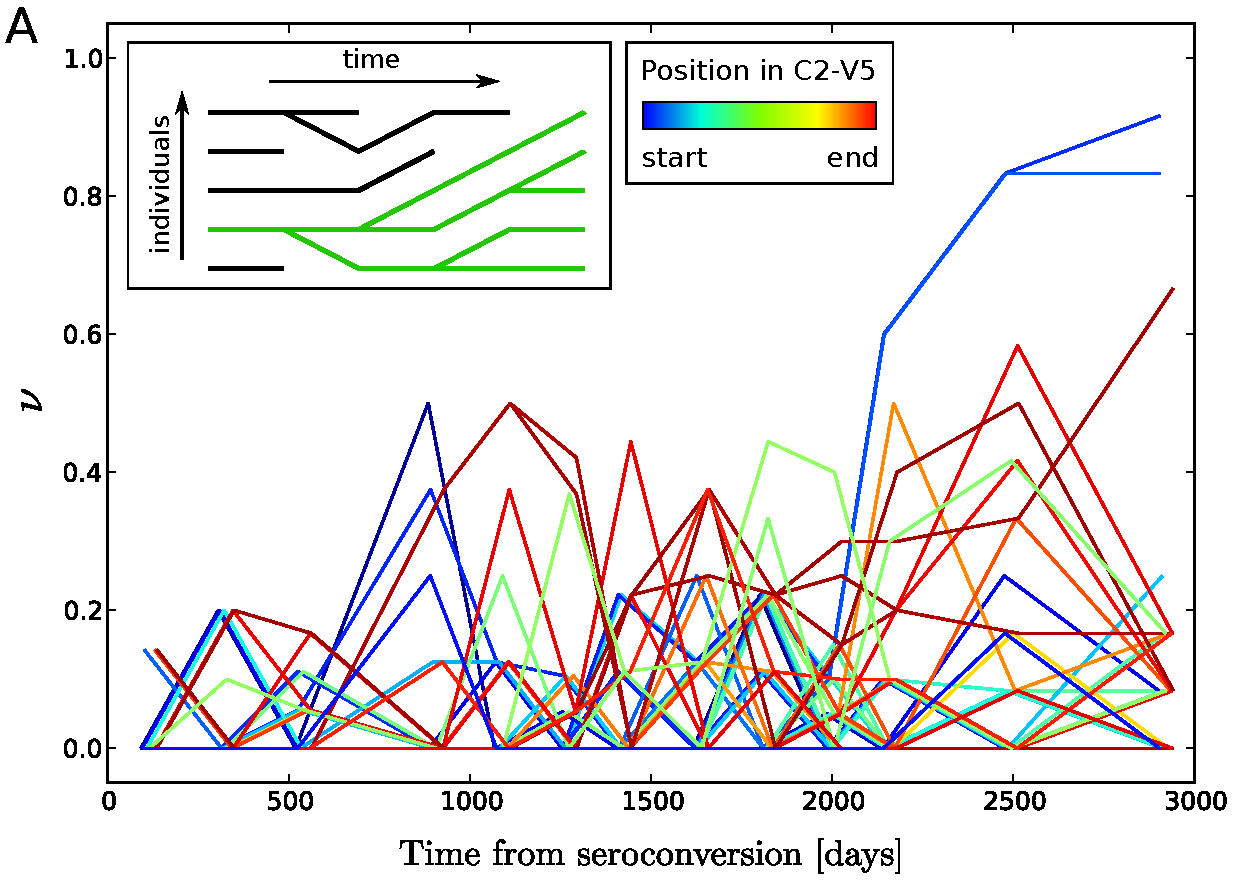
\includegraphics[width=\linewidth]{Shankarappa_allele_freqs_trajectories_syn_p8.pdf}
\label{fig:aftsyn}}\\
\subfloat{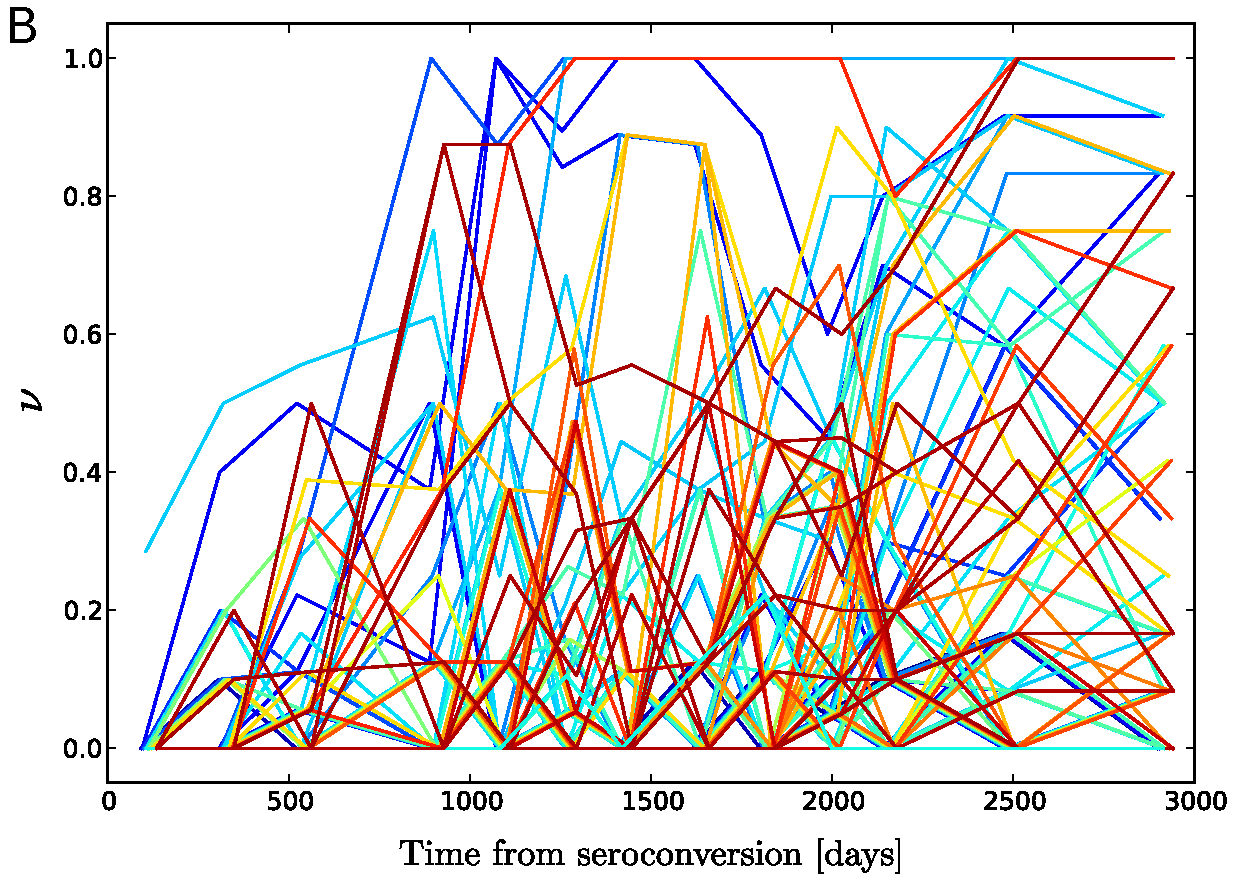
\includegraphics[width=\linewidth]{Shankarappa_allele_freqs_trajectories_nonsyn_p8.pdf}
\label{fig:aftnonsyn}}
\caption{Time series of allele frequencies in \env, C2-V5, from
patient 8~\cite{shankarappa_consistent_1999},
divided by synonymous (panel A) and nonsynonymous (panel B) derived alleles.
While nonsynonymous mutations frequently fix, very few synonymous
mutations do even though they are frequently observed at intermediate
frequencies. Colors indicate the position of the site along the C2-V5 region
(blue to red). Inset: the fixation probability $P_\text{fix}(\nu)$ of a neutral mutation
is simply the likelihood that the future common ancestor is currently carrying
it, i.e. its frequency $\nu$.}
\label{fig:aft}
\end{center}
\end{figure}

When interpreting these results for the fixation probabilities, it is important
to distinguish random mutations, and polymorphisms at a given frequency that has
already been filtered by selection.
A polymorphism could be beneficial to the virus and on its way to fixation. In
this case, we expect that it fixes almost surely given we see it at high
frequency. If, on the other hand, the polymorphism is deleterious it must have
gotten to high frequency by a chance event (genetic drift or hitch-hiking), and
we expect that selection will drive it out of the population again. Hence our
observations suggest that many of the synonymous polymorphisms at intermediate
frequencies in the part of \env~that includes the hypervariable regions are
deleterious, while outside this regions polymorphisms are mostly roughly
neutral. Note that this does not imply that all synonymous mutations are neutral
-- only those mutations observed at high frequencies tend to be neutral.

\begin{figure}
\begin{center}
\subfloat{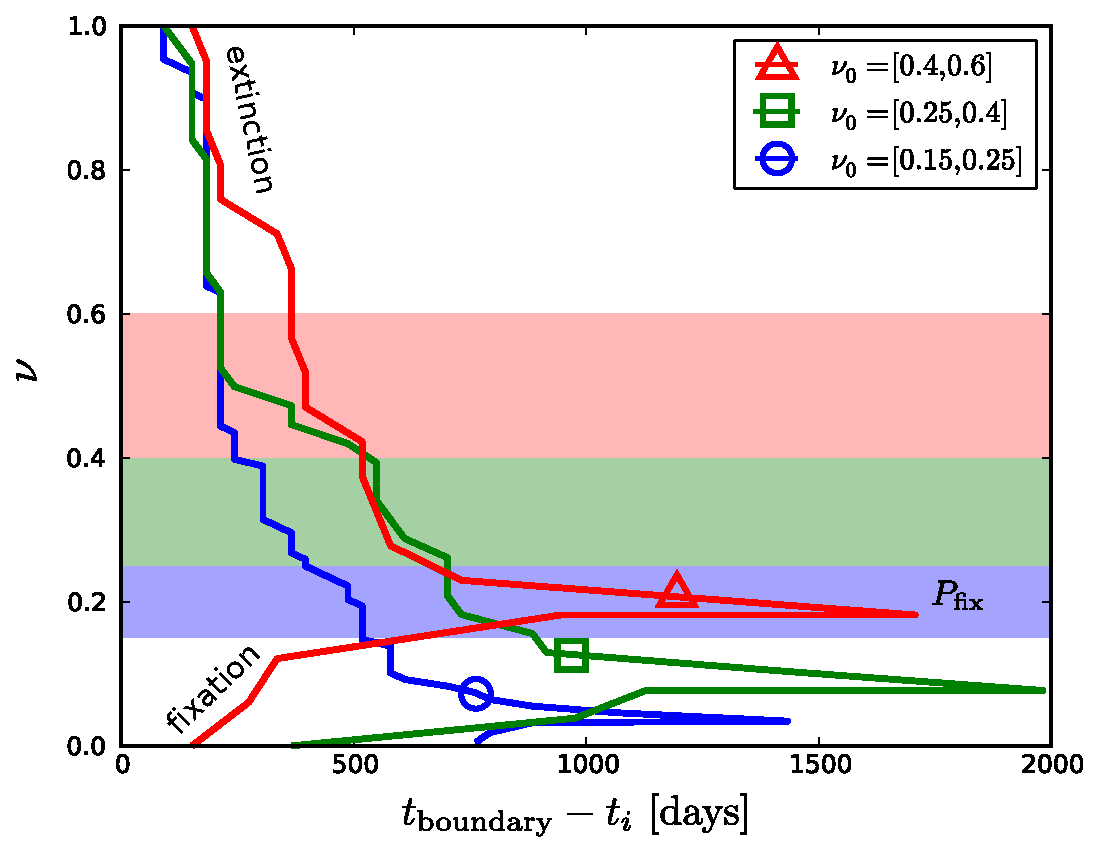
\includegraphics[width=0.9\linewidth]{Shankarappa_fix_loss_dt_times}
\label{fig:fixp1}}\\
\subfloat{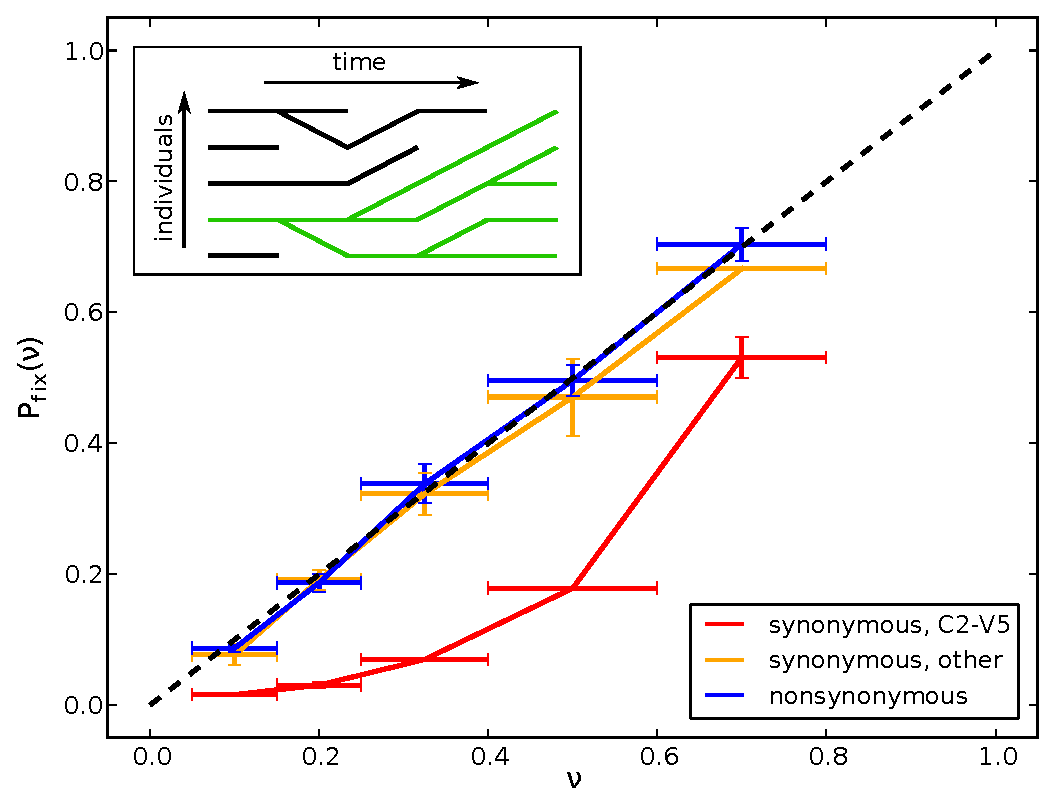
\includegraphics[width=0.9\linewidth]{Bunnik2008_fixmid_syn_ShankanonShanka}
\label{fig:fixp2}}
\caption{(Panel A) Time course of loss and fixation of synonymous mutations
observed in a frequency interval $\nu_0$. The ultimate fraction of synonymous
mutations that fix as a function of intermediate frequency $\nu_0$ is the
fixation probability. (Panel B) Fixation probability of derived synonymous
alleles is strongly suppressed in C2-V5 versus other parts of the {\it env}
gene. The horizontal error bars on the abscissa are bin sizes, the vertical ones
the standard deviation after 100 patient bootstraps of the data. Data from
Refs.~\cite{shankarappa_consistent_1999, bunnik_autologous_2008}.}
\label{fig:fixp}
\end{center}
\end{figure}

\subsection{Synonymous mutations in C2-V5 tend to disrupt conserved RNA stems}

One possible {\it a priori} explanation for lack of fixation of synonymous
mutations in C2-V5 are  secondary structures in the viral RNA. It has
been suggested early on that parts of the viral genome that has the potential to
form stems is better conserved than the
remainder~\citep{forsdyke_reciprocal_1995,snoeck_mapping_2011}.

Recently, the propensity of nucleotides of the HIV genome to form base pairs has
been measured using the SHAPE assay (a biochemical reaction preferentially
altering unpaired bases)~\citep{watts_architecture_2009}. The SHAPE assay has
shown that the variable regions V1 to V5 tend to be unpaired, while the
conserved regions between those variable regions form stems. We partition all
synonymous alleles observed at intermediate frequencies above 10-15\% depending
on their final destiny (fixation or extinction). Subsequently, we align our
sequences to the reference NL4-3 strain used in
ref.~\citep{watts_architecture_2009} and assign them SHAPE reactivities. As
shown in \FIG{SHAPEA} in a cumulative histogram, the reactivities of fixed
alleles (red line) are systematically larger than of alleles that are doomed to
extinction (blue line) (Kolmogorov-Smirnov test, $P\approx 0.002$).
In other words, alleles that are likely to be
breaking RNA helices are also more likely to revert and finally be lost from the
population. As a control, the average over non-observed but potentially
available polymorphisms lies between the two curves (green line), as expected
(because only some of these mutations will interfere with stem loop formation).
To test the hypothesis that mutations in C2-V5 are lost since break stems
in the conserved between the variable loops, we split the synonymous mutations
in the extended V1-V5 region further into conserved and variable regions and
found that the biggest depression in fixation probability is observed in the
conserved stems, while the variable loops show little deviation from the
neutral signature, see \FIG{SHAPEB}. This is consistent with important stem
structures in conservered regions between loops.

In addition to RNA secondary structure, we have considered other possible
explanations for a fitness defect of synonymous mutations, in particular codon
usage bias (CUB). HIV is known to prefer A-rich codons over highly expressed
human codons~\citep{jenkins_extent_2003,kuyl_biased_2012}. We do not find,
however, any evidence for a contribution of CUB to the ultimate fate of
synonymous alleles consistent with the fact that CUB between HIV and human genes
is not shrinking at the macroevolutionary level \citep{kuyl_biased_2012}. 
Furthermore, CUB in the V1-C5 region is not very different from other parts of
the HIV genome, whereas the reduced fixation probability is only observed there. In
conclusion, although we cannot exclude an effect of CUB on fitness as a general
rule, we expect it to be a minor effect in our context. 


\begin{figure}
\begin{center}
\subfloat{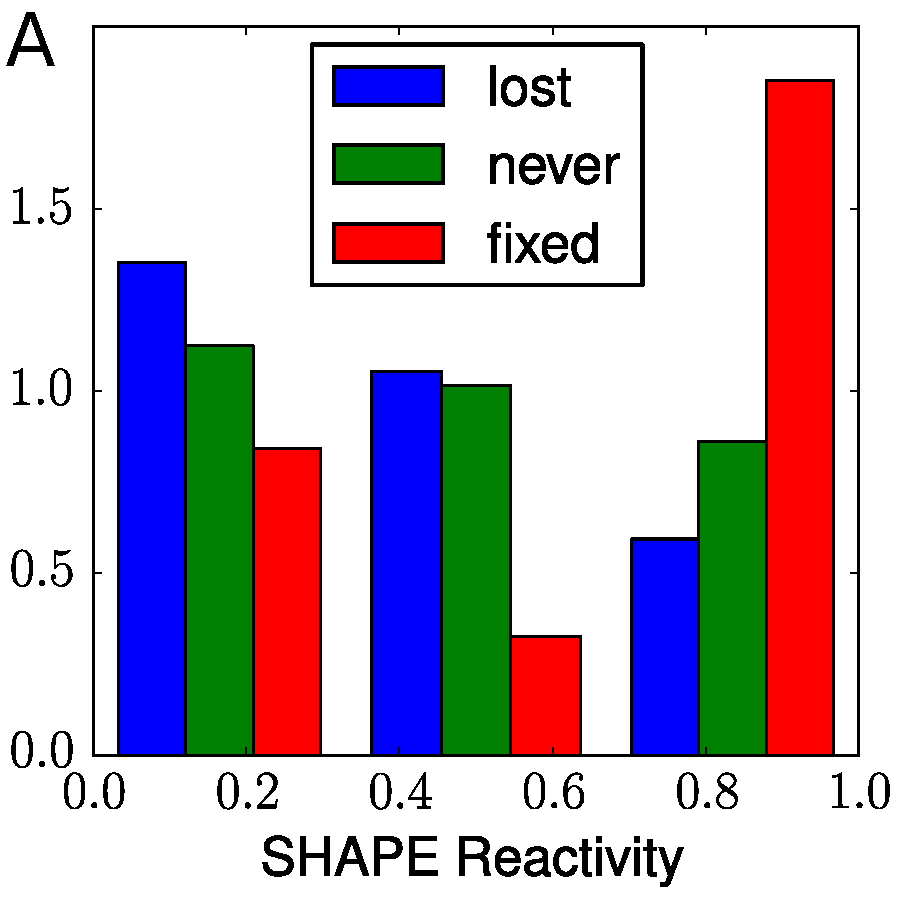
\includegraphics[width=0.9\linewidth]{reactivities_histograms_syn}
\label{fig:SHAPEA}}\\
\subfloat{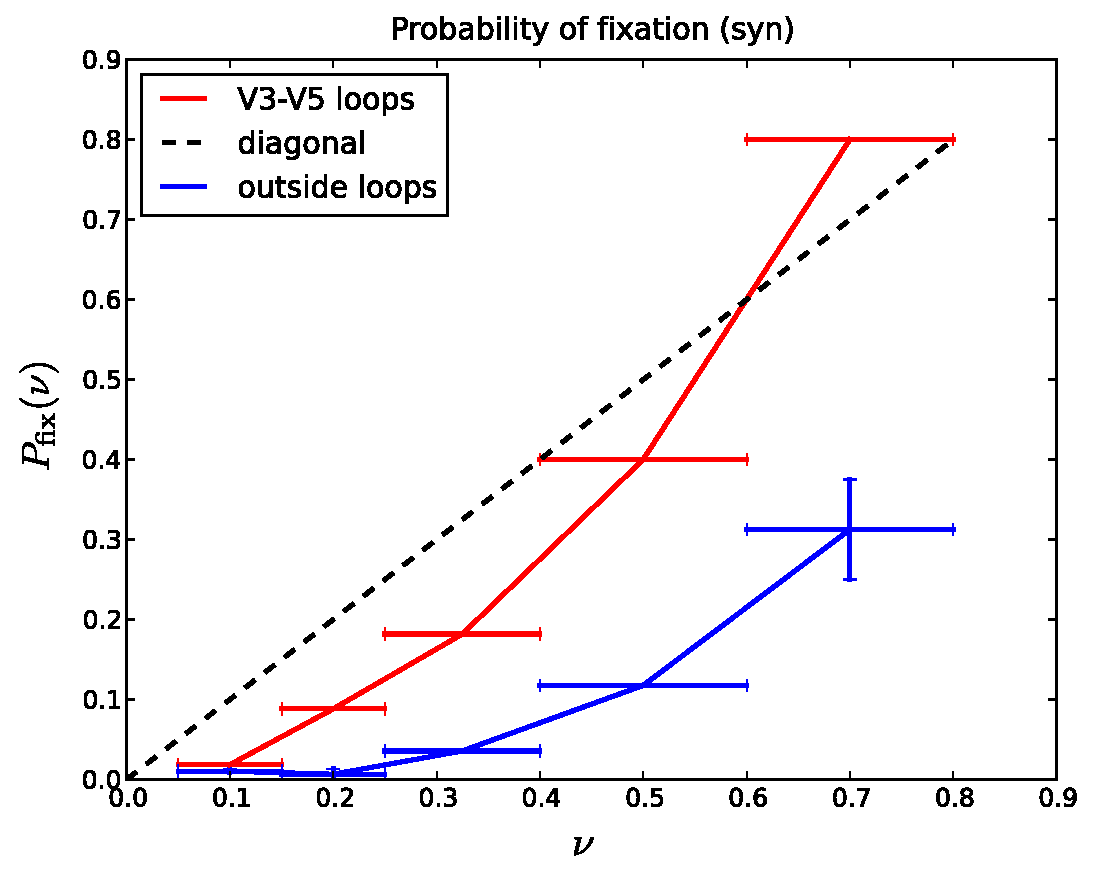
\includegraphics[width=0.9\linewidth]{Shankarappa_fixmid_syn_V_regions.pdf}\label{fig:SHAPEB}}
\caption{Permissible synonymous mutations have
high SHAPE reactivities. \comment{Is this C2-V5 only?} 
Panel A) Synonymous substitions in the C2-V5 region have substantially higher
SHAPE reactivities than mutations that reach frequencies above 15\%, but are
susequently lost. This difference is quantified by a cumulative histogram
($p=0.002$, Kolmogorov-Smirnov two sample test). Mutations that are never
observered show an intermediate distribution of SHAPE values.
Panel B shows the fixation probablility of synonymous mutations in C2-V5
separately for variable loops and the connecting conserved regions, that
harbor conserved RNA stems. As expected, fixation probability is lower inside
the conserved regions. Data from Refs.~\cite{shankarappa_consistent_1999,
bunnik_autologous_2008, liu_selection_2006}.}
\label{fig:SHAPE}
\end{center}
\end{figure}


\subsection{Deleterious mutations are brought to high frequency by hitch-hiking}

While the observation that some fraction of synonymous mutations is deleterious
is not unexpected, it seems odd that we observe them at high population
frequency -- at least in some regions of the genome. The region of \env~ in
which we observe deleterious mutations at high frequency, however, is special in
that it undergoes frequent adaptive changes to evade recognition by neutralizing
antibodies~\cite{williamson_adaptation_2003,richman_rapid_2003}. Due to the limited amount of
recombination in HIV~\cite{neher_recombination_2010,batorsky_estimate_2011},
deleterious mutations that are linked to adaptive variants can reach high
frequency. This process is known as hitch-hiking \citep{smith_hitch-hiking_1974}
or genetic draft \citep{gillespie_genetic_2000,neher_genetic_2011}.

The potential for hitchhiking is already apparent from the allele frequency
trajectories in \FIG{aft}, where many mutations appear to change rapidly in
frequency as a flock. In order
to be advected to high frequency by a linked adaptive mutation, the deleterious
effect of the mutation has to be substantially smaller than the adaptive effect.
The latter was estimated to be on the order of $s_a = 0.01$ per day~\citep{neher_recombination_2010}.
The approximate magnitude of the deleterious effects can be estimated from
\FIG{fixp1}, that shows the distribution of times for synonymous
alleles to reach the fix or get lost starting from intermediate frequencies. The
typical time to loss is of the order of 500 days. If this loss is driven by the
deleterious effect of the mutation, this corresponds to deleterious effects of
roughly $s_d \sim - 0.002$ per day.

\begin{figure}
\begin{center}
\subfloat{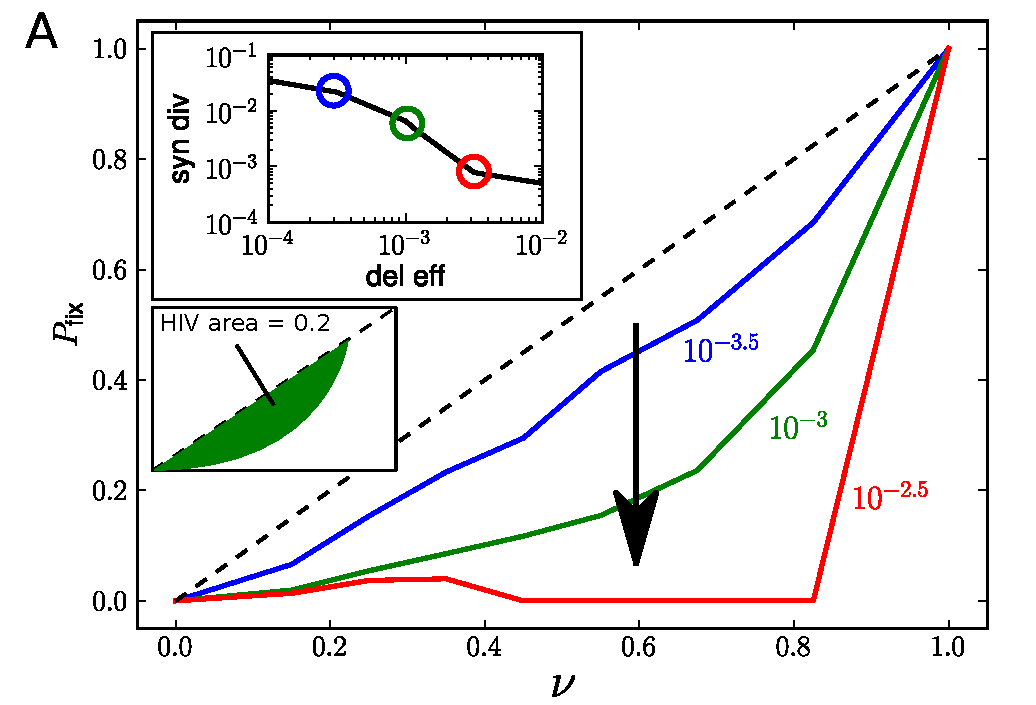
\includegraphics[width=\linewidth]{simulations_graduallydel.pdf}
\label{fig:simfixpvar}}\\
\subfloat{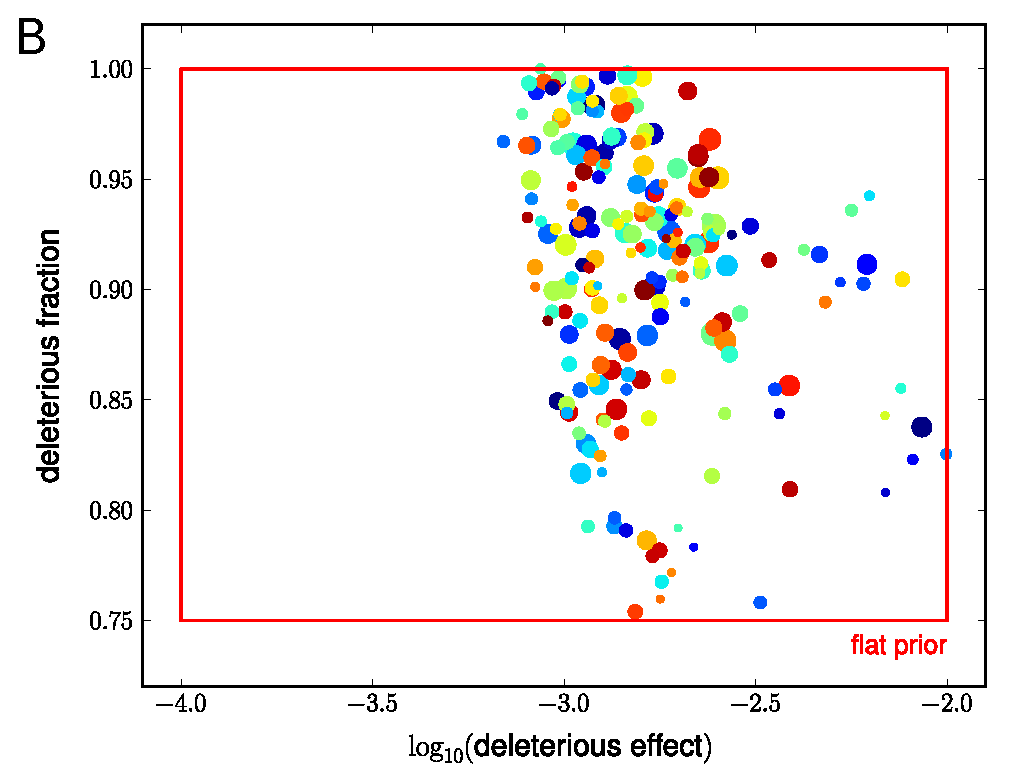
\includegraphics[width=\linewidth]{simulations_syn.pdf}
\label{fig:simsfig}}
\caption{(Panel A) The depression in $P_\text{fix}$ depends on the deleterious
effect size of the synonymous alleles. This parameter also reduces synonymous
diversity, measured by probability of a derived allele to be found at
intermediate frequencies $P_\text{interm}$ (first inset).
(Panel B) To assess the parameter space that affects synonymous fixation and
diversity, we run many simulations with random parameters for deleterious effect
size, fraction of deleterious synonymous sites, average size of escape
mutations (color, blue ($10^{-2.5}$) to red ($10^{-1.5}$)), and rate of
introduction of new epitopes (marker size, from $10^{-3}$ to $10^{-2}$ per
generation). Mostly simulations with small deleterious effects and relatively
high deleterious fractions of synonymous mutations reproduce synonymous HIV-like
fixation probability and diversity. Parameters are chosen uniformly on a
logarithmic scale from the indicated windows. \comment{should we extend the
parameters space maybe to $10^{-4}$?}}
\label{fig:simheat}
\end{center}
\end{figure}

To get a better idea of the range of parameters that are compatible with the
observations and our interpretation, we perform computer simulations of
evolving viral populations assuming a mix of positive and purifying selection
and rare recombination.
For this purpose, we use the simulation package FFPopSim, which includes a
module dedicated to intrapatient HIV evolution~\citep{zanini_ffpopsim:_2012}. 

The first result of the simulations is that genetic draft can indeed bring weakly
deleterious mutations to high frequencies and results in a dependence of the
fixation probability on initial frequency that is compatible with observations
(see \FIG{simfixpvar}).
To assess the reduction in fixation probability quantitatively, we calculate
the area between the measured fixation probability and the diagonal, which is
the neutral expectation (\FIG{simfixpvar}, lower inset). This area spans a range
between $-0.5$ (no fixation at all), zero (neutral-like curve), and $+0.5$ (always
fixed). Furthermore, we quantify synonymous diversity via the probability
$P_\text{interm}$ of a synonymous derived allele to be at intermediate frequencies
$0.25 < \nu < 0.75$ (\FIG{simfixpvar}, top inset).
The HIV data correspond to an area $A_\text{syn} \sim -0.2$  for synonymous
changes and $A_\text{nonsyn} \sim 0$ for nonsynonymous changes,
and a synonymous diversity $P_\text{interm} \sim 0.005$.
In the three simulations shown in \FIG{simfixpvar}, the fixation probability of
synonymous alleles decreases from the neutral expectation ($A_\text{syn} \sim 0$) to zero
($A_\text{syn} \sim -0.5$) as their fitness effect
worsens; the synonymous diversity plummets as well, as it is harder for
deleterious mutations to reach the frequency threshold of 0.25.

To map the parameter range of the model that is compatible with the data, we
repeatedly simulated the evolution with random choices for the deleterious
effect of synonymous mutations, the fraction of synonymous mutations that are
deleterious, the escape rate of adaptive mutations, and the frequency of
escapes.  Among all simulations, we select the ones that show $A_\text{syn}$ and
$P_\text{interm}$ as observed in the data, i.e., a large depression in fixation
probability of synonymous mutations but, simulteneously, a moderately high
synonymous diversity. Specifically, \FIG{simsfig} shows parameter combinations
for which we found $A_\text{syn} < -0.15$ and $0.0025 < P_\text{interm} < 0.010$
(twofold variation around the observed value). This selection imposes a strong
constraint on the deleterious fraction and effect size (see \FIG{simsfig}).
A high fraction ($\gtrsim 0.8$) of only slightly deleterious synonymous sites,
with effect size $|s_d| \sim 0.002$, is required. This result fits well the
expectation based on the fixation/extinction times above (see \FIG{fixp1}).
The results are plausible:
(a) since high frequency bins are enriched in neutral mutations (it is easier
for them to hitchhike), a depression in $\pfix$ will be
visible only if deleterious mutations are pervasive; (b) in order to
hitchhike, the deleterious effect size has to be less than the escape rate, otherwise the
double mutant has little or no fitness advantage; (c) mutations with a 
deleterious effect weaker than approximately $0.001$ behave neutrally
consistent with the typical coalescent times observed in HIV.

As long as only features of synonymous mutations are filtered, as performed
above, no strong correlation of the two nonsynonymous parameters, escape rate
and rate of appearance of epitopes, is observed; in \FIG{simsfig}, the points
shown possess a variety of shapes and colors. In most of these simulations, 
however, nonsynonymous mutations almost always fix once they reach high frequencies
-- their nonsynonymous fixation area is well above zero. This is incompatible
with the blue line in \FIG{fixp}: in an HIV infection, nonsynonymous mutations fix as if they
were neutral. Although there are no doubts that nonsynonymous variation in the
variable regions is driven by positive selection and not by genetic drift, the
biological reason for the neutral-like curve in \FIG{fixp} is unclear.
Inspecting the trajectories of nonsynonymous mutations
suggests the rapid rise and fall of many alleles. We test two possible
mechanisms that are biologically plausible and could explain the transient rise
of nonsynonymous mutations: time-dependent selection and within-epitope
competition.

The former hypothesis can be formulated as follows: if the immune system
recognizes the escape mutant before its fixation, the mutant might cease to be
beneficial and disappear soon, despite its quick initial rise in frequency. In support of this idea,
\citet{richman_rapid_2003, bunnik_autologous_2008} report antibody responses to
escape mutants. These respones are delayed by a few months, roughly matching the
average time needed by an escape mutant to cross frequencies of order one.
In the alternative hypothesis, several different escape
mutations within the same epitope might arise almost simultaneously and start to
spread. Their benefits are not additive, because each of them is
essentially sufficient to escape. As a consequence, several escape mutations rise to
high frequency rapidly, while the one with the smallest cost in terms of replication,
packaging, etc.~is most likely to eventually fix. The emergence of
multiple sweeping nonsynonymous mutations in real HIV infections has been shown
previously~\citep{moore_limited_2009, bar_early_2012}.
We tested both hypotheses in our simulation framework and they both seem to
achieve a reduced, neutral-like fixation probability while maintaining a high
rate of substitutions, compatibly with HIV measurements \comment{Supplementary}.
In real HIV infections, both mechanisms are likely to be playing a role.

\section{Discussion}
Despite several known functional roles for RNA secondary structure in the HIV
genome, synonymous mutations are often used as approximately neutral markers in
evolutionary studies of viruses. We have shown that the majority of synonymous
mutations in the conserved regions C2-C5 of the \env~gene are deleterious.
Comparison with recent biochemical studies of binding propensity of bases in RNA
genome suggest that these mutations are deleterious, at least in part, because they disrupt
stems in RNA secondary structures. Furthermore, we provide evidence that these
mutations are brought to high frequency through linkage to adaptive mutations.
The latter mutations are only transiently adaptive, either through a
coevolution with the immune system or redundant escape within an epitope. 

Our observations and conclusion rely heavily on longitudinal data in which the
dynamics of mutations can be explicitly observed. The fact that deleterious
mutations can be brought to high frequencies through hitchhiking underscores
the intensity of the coevolution with the immune system. The fact that
multiple escape mutations in the same epitope -- as is indeed observed in
studies of antibody escape~\citep{moore_limited_2009, bar_early_2012} -- are
necessary to explain the patterns of fixation of nonsynonymous mutations points
towards a large populations size that rapidly discovers adaptive mutations. A
similar point has been made recently by Boltz {\it et al.} in the context of
preexisting drug resistance mutations~\citep{boltz_ultrasensitive_2012}. 

The observed hitchhiking highlights the importance of linkage due to infrequent
recombination for the evolution of HIV
\citep{neher_recombination_2010,batorsky_estimate_2011,
josefsson_majority_2011}. The recombination rate has been estimated to be on the
order of $\rho = 10^{-5}$ per base and day. It takes roughly $t_{sw} =
\epsilon^{-1} \log \nu_0$ generations for escape mutation with escape rate $\epsilon$ to rise
from an initially low frequency $\nu_0\sim \mu$ to frequency one. This implies
that a region of length $l = (\rho t_{sw})^{-1} = \epsilon / \rho \log \nu_0$
remains linked to the adaptive mutation. With $\epsilon=0.01$, we have $l\approx
100$ bases. Hence we expect strong linkage between the variable loops and their
surrounding stems, but none far beyond the variable regions, consistent with the lack of signal
outside of C1-V5. In case of much stronger selection -- such as observed during
early CTL escape or drug resistance evolution -- the linked  region is of course
much larger \citep{nijhuis_stochastic_1998}.

A functional significance of the insulating RNA structure stems between the
hyper variable loops has been proposed
previously~\citep{watts_architecture_2009, sanjuan_interplay_2011}.
\citet{sanjuan_interplay_2011} have shown that insulating stems are relevant for
viral fitness {\it in vivo}. Our analysis is limited by the availability of
longitudinal data which requires a focus on the the variable regions of \env.
Conserved RNA structures exist in different parts of the HIV genome (several are
known). In absence of repeated adaptive substitutions in the vicinity that cause
hitchhiking, the deleterious synonymous mutations remain at low frequencies and
can only be observed by deep sequencing methods. 

The fixation and extinction times and probabilities represent a rich and simple
summary statistics useful to characterize longitudinal sequence data and compare
to models via computer simulations.
A similar method has been recently used in a longitudinal study of
influenza~\citep{strelkowa_clonal_2012}. The propagators suggested in that
paper, however, represent ratios between nonsynonymous and synonymous mutations.
The latter is used as an approximately neutral control and this method can
therefore not be used to investigate synonymous changes themselves.

Our results emphasize the inadequacy of independent site
models of HIV evolution and the common assumption that selection is time
independent or additive. If genetic variation is only transiently beneficial,
existing methods to quantify selection will yield substantial underestimates
\citep{williamson_adaptation_2003,neher_rate_2010,batorsky_estimate_2011}. To explain the
observations regarding the fixation probabilities of non-synonymous mutations,
either transient selection, or substational within-epitope competition are
necessary. Which mechanism is more widespread is not clear as of now,
there is evidence for both~\citep{richman_rapid_2003, moore_limited_2009,
bar_early_2012}.

\section{Methods}
\subsection{Sequence data collection}
Longitudinal intrapatient viral RNA sequences were collected for published
studies~\citep{shankarappa_consistent_1999,
liu_selection_2006, bunnik_autologous_2008} and downloaded from the Los Alamos
National Laboratory (LANL) HIV sequence database~\citep{LANL2012}. The sequences from
some patients showed signs of HIV compartimentalization into subpopulations and
were discarded; a grand total of 11
patients with approximately 6 time points each and 10 sequences per time point
were analyzed. The time interval or resolution between two consecutive sequences
was approximately 6 to 18 months.

\comment{How did you determine who to discard. Maybe we should include the PCA
plots into the supplement.}


\subsection{Sequence analysis}
The good sequences were aligned within each patient
via the translated amino acid sequence, using
Muscle~\citep{edgar_muscle:_2004}, and to the NL4-3 reference sequence used
by \citet{watts_architecture_2009} in the SHAPE assay. Within each patient, a
consensus RNA sequence at the first time point was used to classify alleles as ancestral or
derived at all sites. Problematic sites that included large frequencies of gaps
were excluded from the analysis to avoid artefactual substitutions due to
alignment errors. Time series of allele frequencies were extracted from the
sequences.

The synonymity of a mutation was assigned if the rest of the codon was
in the ancestral state and using the standard genetic code. Cases where more
than one mutation within the codon was observed were discarded. Slightly
different criteria for synonymous/nonsynonymous discrimination yielded similar
results.

\subsection{Fixation probability and secondary structure}
For the estimate of times to fixation/extinction, polymorphisms were
binned by frequency and the time to reaching the first boundary (fixation or
extinction) was stored. For the fixation probability, the long-time limit of the
resulting curves was used, excluding polymorphisms that arose late in the
clinical history (and would have had no time to reach either boundary).

For the correlation analysis with RNA secondary structure, the SHAPE scores were
downloaded from the journal website~\citep{watts_architecture_2009}. By virtue
of the alignment of the longitudinal sequences with the reference used by
\citet{watts_architecture_2009}, SHAPE reactivities were assigned to most sites.
Problematic assignments in indel-rich regions were excluded from the analysis.
In order to restrict the analysis to synonymous polymorphisms, a lower frequency
threshold of 0.15 was used (other thresholds yielded the same results). Since
very few polymorphisms hitchhike beyond, say, a frequency of 0.5, this pool is
enriched for to-be-lost mutations; hence the ``lost" curve in \FIG{SHAPEA}
contains much more points than the ``fixed" one.

The V loops and flanking regions were identified manually starting from the
annotated reference HXB2 sequence from the LANL HIV database~\citep{LANL2012}. A
similar approach was used to label the C2-V5 region sequenced in
ref.~\citep{shankarappa_consistent_1999}.

\subsection{Computer simulations}
Simulations were performed using the recently published software
FFPopSim~\citep{zanini_ffpopsim:_2012}. Both full-length HIV genomes and
\env{}-only simulations were performed and yielded comparable results. For each
set of parameters, approximately 100 simulation runs were averaged over. In each
run, a random fitness landscape with specified statistical properties (e.g.
density of beneficial sites, average deleterious effect of synonymous changes) was generated.
Although the curves shown in \FIG{simfixpvar} are not very smooth, small
parameter changes resulted in overall consistent trends across many repetitions.

For the discussion of simulation parameters, the areas below or above the neutral
diagonal were estimated from the binned fixation probabilities using the linear
interpolation between the bin centers. This measure is sufficiently precise for
our purposes, because the HIV data are quite scarse themselves.

\section*{Acknowledgements}
\comment{to be written\dots}


%%%%%%%%%%%%%%%%%%%%%%%%%%%%%%%%%%%%%%%%%%%%%%%%%%%%%%%%%%%%%%%%%%%%%%%%%
\bibliographystyle{natbib}
\bibliography{bib}
%%%%%%%%%%%%%%%%%%%%%%%%%%%%%%%%%%%%%%%%%%%%%%%%%%%%%%%%%%%%%%%%%%%%%%%%%
\end{document}
%%%%%%%%%%%%%%%%%%%%%%%%%%%%%%%%%%%%%%%%%%%%%%%%%%%%%%%%%%%%%%%%%%%%%%%%%

